\documentclass[12pt]{article}
\usepackage{graphicx}
\usepackage{subcaption}
\usepackage{mwe}
%\usepackage{lingmacros}
%\usepackage{tree-dvips}
%\usepackage{blindtext}
\usepackage[utf8]{inputenc}
\usepackage[T1]{fontenc}

\usepackage{algorithmicx}
\usepackage{algpseudocode}

\usepackage[inline]{enumitem}

\usepackage{tikz}
\usetikzlibrary{positioning}

\begin{document}

\title{
	Project 3: Neural Transliteration
}
\author{
Gudjon Magnusson 
\and Irina Yakubinskaya 
\and Matthew Goldberg
}

\maketitle

%%%%%%%%%%%%%%%%%%%%%%%%%%%%%%%
%%%%%%%%%%%%%%%%%%%%%%%%%%%%%%%

\section{Seq-to-seq model configuration}

\subsection{Q1}

\begin{figure}[!h]
\centering


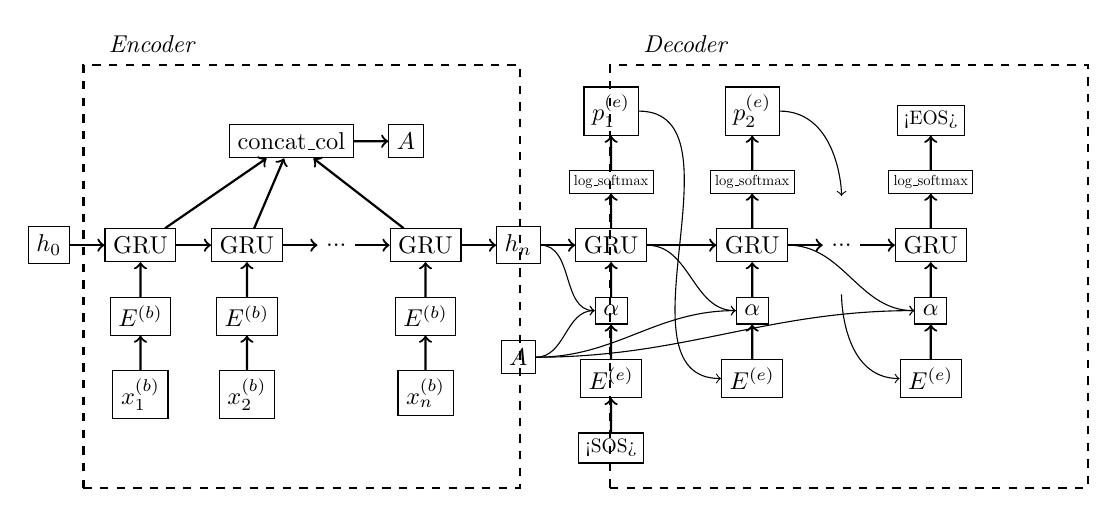
\begin{tikzpicture}[node distance=0.5cm, auto]

\begin{scope}[scale=0.88, transform shape]

	%% Decoder
	\node[draw] (h_0) {$h_0$};
	\node[draw] (gru_f1) [right =of h_0]{GRU};
	\node[draw] (gru_f2) [right =of gru_f1]{GRU};
	\node (gru_fblank) [right =of gru_f2]{...};
	\node[draw] (gru_fn) [right =of gru_fblank]{GRU};

	\draw [->,thick] (h_0) edge (gru_f1);
	\draw [->,thick] (gru_f1) edge (gru_f2);
	\draw [->,thick] (gru_f2) edge (gru_fblank);
	\draw [->,thick] (gru_fblank) edge (gru_fn);

	\node[draw] (ef_1) [below =of gru_f1] {$E^{(b)}$};
	\node[draw] (ef_2) [below =of gru_f2] {$E^{(b)}$};
	\node[draw] (ef_n) [below =of gru_fn] {$E^{(b)}$};
	\draw [->,thick] (ef_1) edge (gru_f1);
	\draw [->,thick] (ef_2) edge (gru_f2);
	\draw [->,thick] (ef_n) edge (gru_fn);

	\node[draw] (f_1) [below =of ef_1] {$x^{(b)}_1$};
	\node[draw] (f_2) [below =of ef_2] {$x^{(b)}_2$};
	\node[draw] (f_n) [below =of ef_n] {$x^{(b)}_n$};
	\draw [->,thick] (f_1) edge (ef_1);
	\draw [->,thick] (f_2) edge (ef_2);
	\draw [->,thick] (f_n) edge (ef_n);

	\node[draw] (cat_f) at (3.5, 1.5) {concat\_col};
	\node[draw] (A_f) [right =of cat_f] {$A$};
	\draw [->,thick] (cat_f) edge (A_f);
	\draw [->,thick] (gru_f1) edge (cat_f);
	\draw [->,thick] (gru_f2) edge (cat_f);
	\draw [->,thick] (gru_fn) edge (cat_f);

	\node at (1.5, 2.9) {\textit{Encoder}};
	\draw[thick,dashed] (0.5, -3.5) -- (6.8, -3.5) -- (6.8, 2.6) -- (0.5, 2.6) -- (0.5, -3.5);

	%% Middle
	\node[draw] (h_n) [right =of gru_fn]{$h_n$};
	\draw [->,thick] (gru_fn) edge (h_n);

	%% Encoder
	\node[draw] (gru_e1) [right =of h_n]{GRU};
	\node[draw] (gru_e2) [right = 1.0cm of gru_e1]{GRU};
	\node (gru_eblank) [right =of gru_e2]{...};
	\node[draw] (gru_en) [right =of gru_eblank]{GRU};
	\draw [->,thick] (h_n) edge (gru_e1);
	\draw [->,thick] (gru_e1) edge (gru_e2);
	\draw [->,thick] (gru_e2) edge (gru_eblank);
	\draw [->,thick] (gru_eblank) edge (gru_en);

	\node[draw, scale=0.6] (log_e1) [above =of gru_e1]{log\_softmax};
	\node[draw, scale=0.6] (log_e2) [above =of gru_e2]{log\_softmax};
	\node[draw, scale=0.6] (log_en) [above =of gru_en]{log\_softmax};
	\draw [->,thick] (gru_e1) edge (log_e1);
	\draw [->,thick] (gru_e2) edge (log_e2);
	\draw [->,thick] (gru_en) edge (log_en);

	\node[draw] (p_1) [above =of log_e1]{$p^{(e)}_1$};
	\node[draw] (p_2) [above =of log_e2]{$p^{(e)}_2$};
	\node[draw, scale=0.8] (p_n) [above =of log_en]{<EOS>};
	\draw [->,thick] (log_e1) edge (p_1);
	\draw [->,thick] (log_e2) edge (p_2);
	\draw [->,thick] (log_en) edge (p_n);

	\node[draw] (att_1) [below =of gru_e1]{$\alpha$};
	\node[draw] (att_2) [below =of gru_e2]{$\alpha$};
	\node[draw] (att_n) [below =of gru_en]{$\alpha$};
	\draw [->,thick] (att_1) edge (gru_e1);
	\draw [->,thick] (att_2) edge (gru_e2);
	\draw [->,thick] (att_n) edge (gru_en);

	\node[draw] (ee_1) [below =of att_1]{$E^{(e)}$};
	\node[draw] (ee_2) [below =of att_2]{$E^{(e)}$};
	\node[draw] (ee_n) [below =of att_n]{$E^{(e)}$};
	\draw [->,thick] (ee_1) edge (att_1);
	\draw [->,thick] (ee_2) edge (att_2);
	\draw [->,thick] (ee_n) edge (att_n);

	\node[draw, scale=0.8] (sos) [below =of ee_1]{<SOS>};
	\draw [->,thick] (sos) edge (ee_1);

	\draw[->] (p_1) to[in=180,out=0] (ee_2);
	\draw[->, shorten >=0.5cm] (p_2) to[in=90,out=0] (gru_eblank);
	\draw[->, shorten <=0.5cm] (gru_eblank) to[in=180,out=270] (ee_n);

	\node[draw] (A_e) [below = 1.1 of h_n]{$A$}; % at (8, -1.5)
	\draw[->] (A_e) to[in=180,out=0] (att_1);
	\draw[->] (A_e) to[in=180,out=0] (att_2);
	\draw[->] (A_e) to[in=180,out=0] (att_n);

	\draw[->] (h_n) to[in=180,out=0] (att_1);
	\draw[->] (gru_e1) to[in=180,out=0] (att_2);
	\draw[->] (gru_e2) to[in=180,out=0] (att_n);

	\node at (9.2, 2.9) {\textit{Decoder}};
	\draw[thick,dashed] (8.1, -3.5) -- (15.0, -3.5) -- (15.0, 2.6) -- (8.1, 2.6) -- (8.1, -3.5);

\end{scope}

\end{tikzpicture}

\caption{Computation graph of the encoder-decoder model}
\label{fig_compgraph}
\end{figure}

Figure \ref{fig_compgraph} shown an overview of how the model works. The attention mechanism is simplified to fit it in the graph and is represented by the unit $\alpha$. The attention score is computed using the bilinear method. A linear transformation is applied to the encoder embedding before computing the dot product with the decoder embedding.

$h_i$ is the hidden layer at timestep $i$. It is a vector of size 256. $h_0$ is initialized as all zeros.

$x_i$ represents the letter at position $i$ in the input word. It is used to lookup a character embedding in the embedding matrix $E$. $E^{(b)}$ is the embedding matrix for the input language, in this case Bulgarian written in the Cyrillic alphabet. $E^{(b)}$ has size $256 \times 85$. 85 different characters (including start and end tokens), each represented by an embedding of size 256. $E^{(e)}$ is the embedding matrix for the output language and has size $256 \times 31$.

The output at each timestep in the encoder is concatenated to form a matrix $A$ which has size $256 \times n$, where $n$ is the length of the input word. The implementation uses a fixed size matrix with 20 columns but only the first $n$ have non-zero values. Words longer than 20 are filtered out of the training set.
The matrix $A$ is used in the decoder for the attention mechanism.


%%%%%%%%%%%%%%%%%%%%%%%%%%%%%%%

\section{Training algorithm}

\subsection{Q2}

\paragraph{n\_iters} is the number of training iterations used to train the model. Each iteration trains trains the model on one randomly chosen example from the training data.

\paragraph{learning\_rate} is how much the weights are updated based on one example. Before the error gradient is subtracted from the weights, its multiplied by \texttt{learning\_rate}. Slowing down the learning (with $learning\_rate < 1$) makes the process more stable and prevents one bad example from ruining good weights.


\subsection{Q3}

To choose values for \texttt{learning\_rate}, commonly refereed to as $\alpha$, and \texttt{n\_iter} we ran two experiments. 
First we trained the model with a a few different values for \texttt{learning\_rate} and tracked the loss for each iteration. We would like to find a value that decays the loss quickly and appears stable over a large number of iterations.
Figure \ref{fig_learning_rate} shows the comparison of learning curves for a few different values of $\alpha$. In general higher values of $\alpha$ lead to faster convergence, but we found that the training becomes unstable when we raise $\alpha$ to 0.02 or higher. 

Next we trained the model and tracked how the average edit distance on a small held out dataset changed after every 100 iterations. For this we fixed \texttt{learning\_rate} to something that appeared reasonable, we choose 0.01. The goal is to see how long we can train the model before over-fitting.

\begin{figure}[t!]
    \begin{subfigure}[t]{0.5\textwidth}
        \centering
        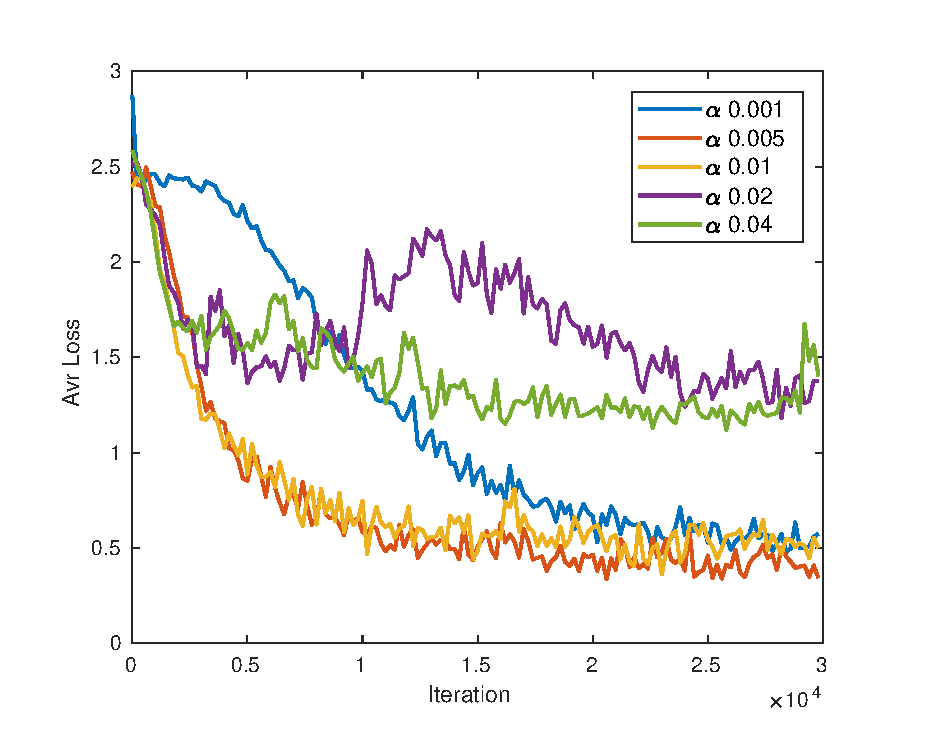
\includegraphics[width=\linewidth]{img/learning_rate2.eps}
        \caption{Learning curves for different $\alpha$}
        \label{fig_learning_rate}
    \end{subfigure}
    \begin{subfigure}[t]{0.5\textwidth}
        \centering
        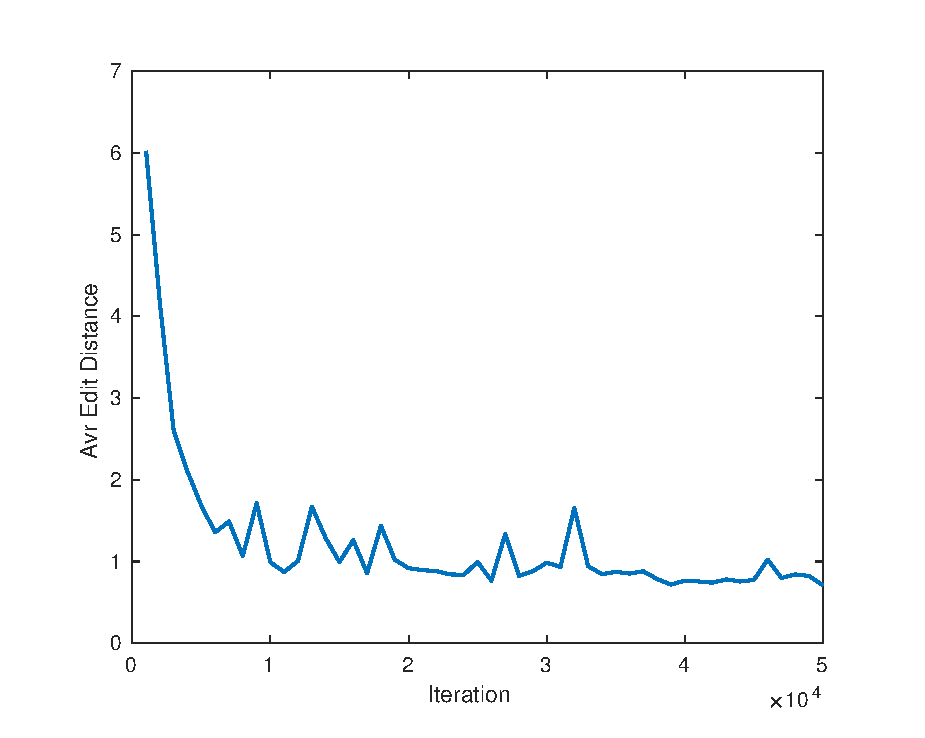
\includegraphics[width=\linewidth]{img/n_iter2.eps}
        \caption{Average edit distance}
        \label{fig_n_iter}
    \end{subfigure}
	\caption{Experiments with \texttt{learning\_rate} and \texttt{n\_iter}}
	\label{fig_train_param}
\end{figure}

We expected to see the edit distance to get lower at first and then start to rise again at some point, but as can be seen in figure \ref{fig_n_iter} the edit distance does not go back up. The score appears to plateau after about 15 thousand iterations, so there is little benefit to train past that.

\section{Understanding teacher forcing}

\subsection{Q4}

\texttt{teacher\_forcing} is the probability of using the "teacher" for each training sample. If it is set to 1, the teacher is used on every sample.

When the teacher is used for training mistakes that the model makes are ignored. At each time step, if the model makes a mistake, it contributes to loss but the model prediction is replaced the with the correct letter. The training moves to the next time step as if no mistake was made.

If the teacher is used too much it can lead to an unstable model that learns how to create good looking outputs rather than good transliterations. I.e its better to get the correct transliteration with one spelling mistake, than the wrong word perfectly spelled.

\subsection{Q5}
 
With higher values of \texttt{teacher\_forcing} the loss decays faster during training. This can be seen in figure \ref{fig_teacher}, which shows the learning curve for 3 different values of \texttt{teacher\_forcing}.

Although it converges faster with higher \texttt{teacher\_forcing}, the average edit distance is lower for the model that was trained with a lower \texttt{teacher\_forcing}. 

\begin{figure}[h]
    \centering
    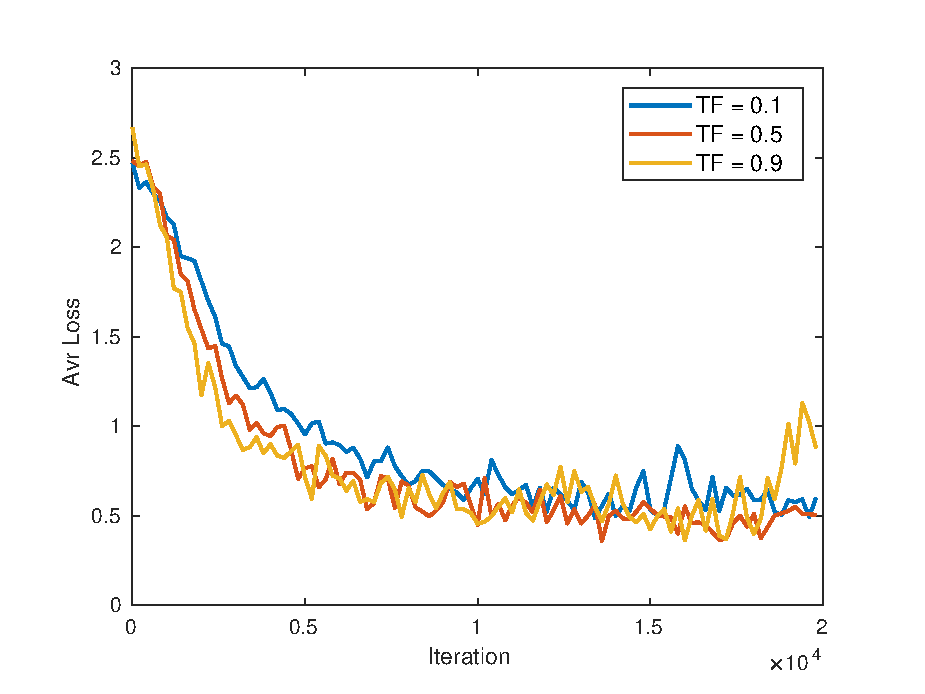
\includegraphics[width=\linewidth]{img/teacher_forcing2.eps}
    \caption{Learning curves for different values of \texttt{teacher\_forcing}}
    \label{fig_teacher}
\end{figure}

\begin{center}
 \begin{tabular}{|c || c | c | c | c | c |} 
 \hline
 \texttt{teacher\_forcing} & 0.0 & 0.1 & 0.5 & 0.9 & 1.0 \\ [0.5ex] 
 \hline
 Avg Edit Dist & 1.12 & 1.09 & 0.77 & 2.43 & 1.16 \\ 
 \hline
\end{tabular}
\end{center}

%%%%%%%%%%%%%%%%%%%%%%%%%%%%%%%

\section{Impact of attention mechanism}

\subsection{Q6}

Transliteration is not a simple one-to-one character replacement, there is a complicated relationship between the input and output characters. The attention mechanism helps to capture that relationship. At each timestep in prediction the model can focus on the input characters that are most likely to influence the output.


\subsection{Q8}

Figure \ref{fig_attention} shows the learning curve for the model with and without the attention mechanism. The model converges faster with attention, and it performs better when evaluated on unseen data. The average edit distance is about 2.4 without attention and 1.72 with attention.

\begin{figure}[h]
    \centering
    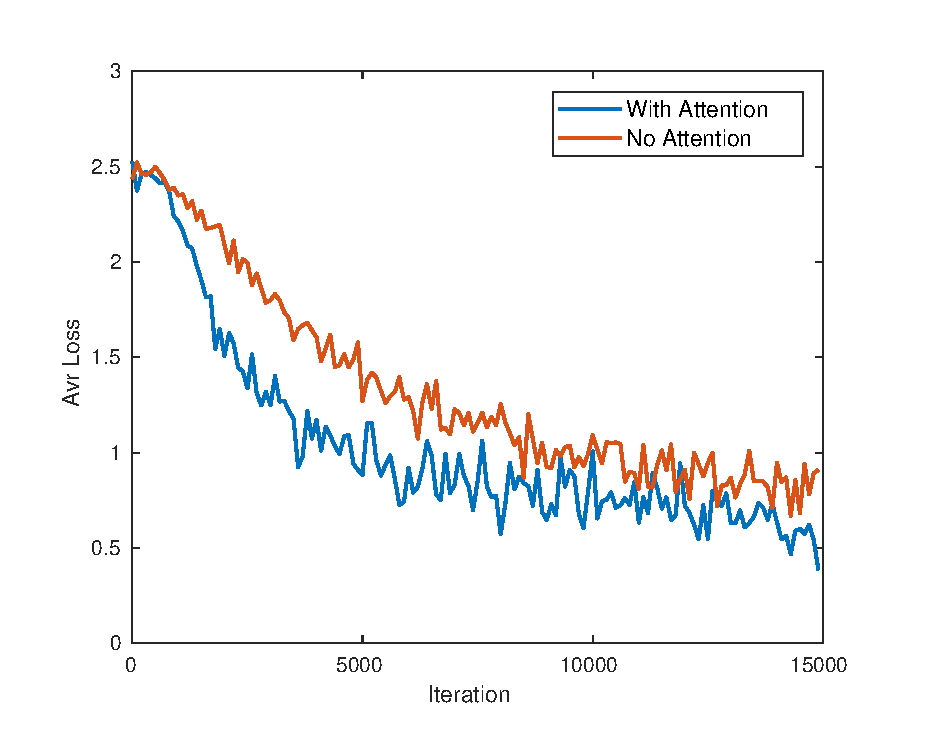
\includegraphics[width=\linewidth]{img/attention2.eps}
    \caption{Learning curves with and without the attention mechanism}
    \label{fig_attention}
\end{figure}

%with attention 1.72
%without 2.4

%%%%%%%%%%%%%%%%%%%%%%%%%%%%%%%

\section{Something new}

\subsection{Q9}
\textit{Briefly explain what you did}

\subsection{Q10}
\textit{Design an experiment to test whether your solution successfully addresses the problem}

\subsection{Q11}
\textit{}


\end{document}